\documentclass{article}
\usepackage[utf8]{inputenc}
\usepackage{graphicx}
\graphicspath{ {./images/} }
\usepackage{multicol}
\usepackage[spanish, english]{babel}
\usepackage[left=3cm,right=3cm,top=3cm,bottom=3cm]{geometry}

\usepackage{multirow} 

\providecommand{\keywords}[1]{
  \small	
  \textbf{\textit{\quad \quad Keywords: }} #1}

\providecommand{\pclave}[1]{
  \small	
  \textbf{\textit{\quad \quad Palabras Clave: }} #1}
\usepackage{fancyhdr} 
\pagestyle{fancy} 
\fancyhead{} 
\fancyfoot{} 
\fancyhead[C]{COMPARATIVE DATAWAREHOUSE VS DATALAKE  $\bullet$ April 2022 $\bullet$ } 
\fancyfoot[RO,LE]{\thepage}

%Idiomas: \selectlanguage{english} \selectlanguage{spanish}

\begin{document}

\title{Encharged Job N°3: COMPARATIVE DATAWAREHOUSE VS DATALAKE}
\begin{titlepage}
\begin{figure}[htb]
\begin{center}

\includegraphics[width=5cm]{logo.png}
\end{center}
\end{figure}
\vspace*{-0.25in}
\begin{center}
\large{UNIVERSIDAD PRIVADA DE TACNA}\\
\vspace*{-0.025in}
INGENIERIA DE SISTEMAS  \\

\vspace*{0.5in}
\begin{large}
TITULO:\\
\end{large}

\vspace*{0.1in}
\begin{Large}
\textbf{COMPARATIVE DATAWAREHOUSE VS DATALAKE} \\
\end{Large}

\vspace*{0.3in}
\begin{Large}
\textbf{COURSE:} \\
\end{Large}

\vspace*{0.1in}
\begin{large}
INTELIGENCIA DE NEGOCIOS\\
\end{large}

\vspace*{0.3in}
\begin{Large}
\textbf{TEACHER:} \\
\end{Large}

\vspace*{0.1in}
\begin{large}
 Ing. Patrick Cuadros Quiroga\\
\end{large}

\vspace*{0.2in}
\vspace*{0.1in}
\begin{large}

MEMBERS: \\
\begin{flushleft}
Briset Celia Garcia Salazar\hfill(2018062496) \\
Diego Manuel Gorbeño Mamani\hfill(2018000354)\\
Luis Fernando Flores Querie\hfill(2018062394)\\

\end{flushleft}
\end{large}

\vspace*{0.1in}
\begin{large}
Tacna - Perú\\
2022
\end{large}
\end{center}
\end{titlepage}

\vspace*{\fill}
	
\begin{center}
    
\selectlanguage{english}
\begin{abstract}
The continuous evolution of business systems has contributed, also through digital transformation processes, to the introduction and optimization of new technologies dedicated to business analytics.

The main objective is to lead the change within a market in continuous and sudden growth, through the adoption of new technologies that include Big Data, Artificial Intelligence processes, Machine Learning and the increasingly requested business Data Lakes.

In recent years, especially thanks to the consolidation of cloud services (mainly AWS and Azure), the paradigm related to reporting systems has continued to evolve, introducing new concepts and architectures that merge technologies related to Data Lake, Big Data and Data Warehouse.
\quad 

 \end{abstract}
 
 
 \keywords{}
 
Big Data, Machine Learning
\end{center}
\vspace*{\fill}

\newpage 


\begin{multicols}{2}

\section{Introduction}
As more companies rely on data to drive critical business decisions, improve product offerings, and better serve customers, the amount of data companies are capturing is greater than ever.
Data warehouses and data lakes have been the most widely used storage architectures for big data.
Depending on your business needs, understanding the different big data warehousing techniques is critical to developing a robust data warehousing pipeline for business intelligence (BI), data analytics, and machine learning (ML) workloads.
In this article we will see the advantages, disadvantages and differences between them.
 
\section{State of Art}

\subsection{Datawarehouse}
Data warehouses pull data from multiple sources and transform and cleanse the data before loading it into the storage system to serve as a single source of truth. Organizations invest in data warehouses because of their ability to quickly deliver business insights from across the organization to help make more informed decisions based on their data.
Data warehouses enable business analysts, data engineers, and decision-makers to access data via BI tools, SQL clients, and other less advanced analytics applications.

The DWH architecture is made up of:
\begin{enumerate}
\item Data sources
\item ETL
\item Data store
\item Dating marts
\item Data exploitation
\end{enumerate}
\\\
\\\
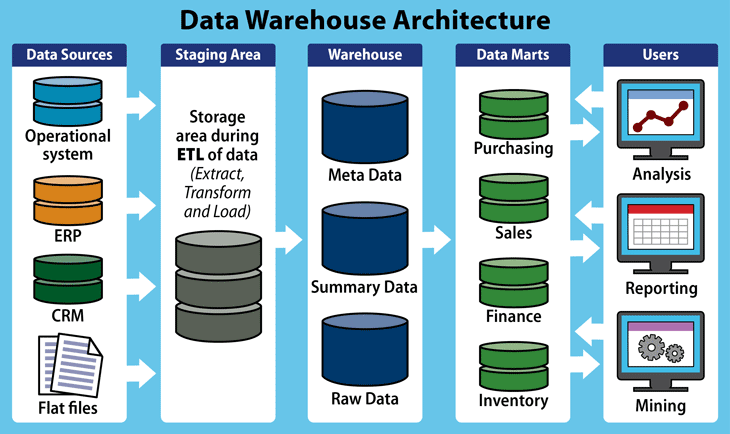
\includegraphics[width=7.5cm]{images/dataWarehouse.png}
\\\
\\\
The important functions which are needed to perform are:
\begin{enumerate}
\item Data Extraction
\item Data Cleaning
\item Data Transformation
\item Data Loading and Refreshing
\end{enumerate}

\subsubsection {Data Warehouse Examples}
\begin{itemize}
\item \textbf{for retailers}, it can help identify customer demographics, identify buying patterns, and improve direct mail responses.
\item \textbf{for banks}, it can aid in credit card fraud detection, help identify the most profitable customers, and highlight the most loyal customers.
\item \textbf{telecommunications companies}, They use it to predict which customers are most likely to switch companies and then give them special incentives to stay.
\item \textbf{insurance companies}, They use it for claims analysis to see which procedures are claimed and to identify patterns of customer risk.
\item \textbf{Los fabricantes}, they can use it to compare the costs of each of their product lines over the past several years, determine what factors drive increases, and see what effect these increases had on overall margins.
\end{itemize}

\subsubsection {The benefits of a data warehouse}
 Some of the benefits include:
\begin{itemize}
\item Offers historical insight into information
\item Increases revenue generation
\item Scalable, flexible, and efficient
\item Easy interoperability with on-premises and cloud-based infrastructure
\item Enhances data security and conformance
\item Offers augmented business intelligence
\item It Helps organizations focus with confidence
\item Streamlines information flow
\end{itemize}

 
\subsubsection{The disadvantages of a data warehouse}
The following problems can be associated with data warehousing:
\begin{itemize}
\item Underestimation of data loading resources
\item Hidden problems in source systems
\item Data homogenization
\end{itemize}





\subsection{Data Lake}
As the data lake definition suggests, a data lake is a huge storage repository that has ample raw data in its basic format. Just like there are multiple tributaries that get in water into lakes, there are multiple sources from where real-time data comes into data lakes. The data could be structured, semi-structured, or unstructured. It is highly flexible, has no fixed limit on size, and is used maximum by data scientists and engineers. It stores all the data irrespective of whether it is needed or not. It provides a huge amount of quantity of data for enhanced performance and native integration.
\begin{center}
	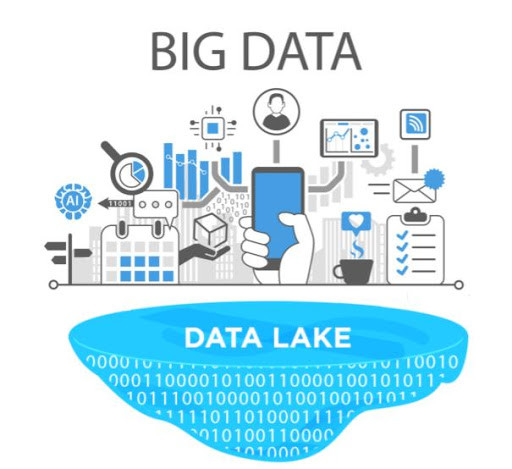
\includegraphics[width=8cm]{./images/datalake.jpg} 
\end{center}
\subsubsection {The benefits of a data Lake}
Some of the benefits include:
\begin{itemize}
\item allow companies immediate access to all data.
\item Data hosted in a data lake is not limited to relational or transactional data.
\item avoid the need to transfer data
\item Reduces long-term cost of ownership
\item Easily adaptable to changes
\item The main advantage of a data lake is the possibility to centralize different sources of content
\end{itemize}

\subsubsection {The disadvantages of a data lake}
some are:
\begin{itemize}
\item Unknown area of data processing
\item Privacy issues
\item The problem of integration
\item The biggest risk of data lakes lies in security and access control
\end{itemize}

\subsubsection {Some of the largest data lakes}
\begin{itemize}
\item AMAZON: Through Amazon S3 and AWS (Amazon Web Services) Lake Formation we can build, protect and manage our data lake.
\begin{center}
	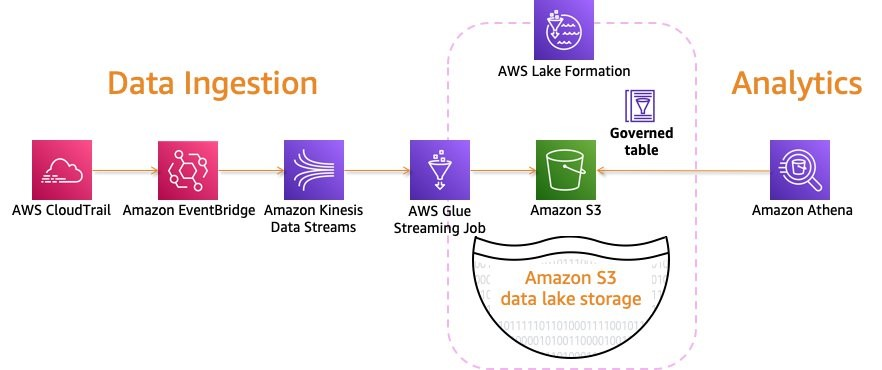
\includegraphics[width=8cm]{./images/AMAZON.jpg} 
\end{center}
\item GOOGLE: Google is another company that offers a data lake service from its Google Cloud Platform.
\begin{center}
	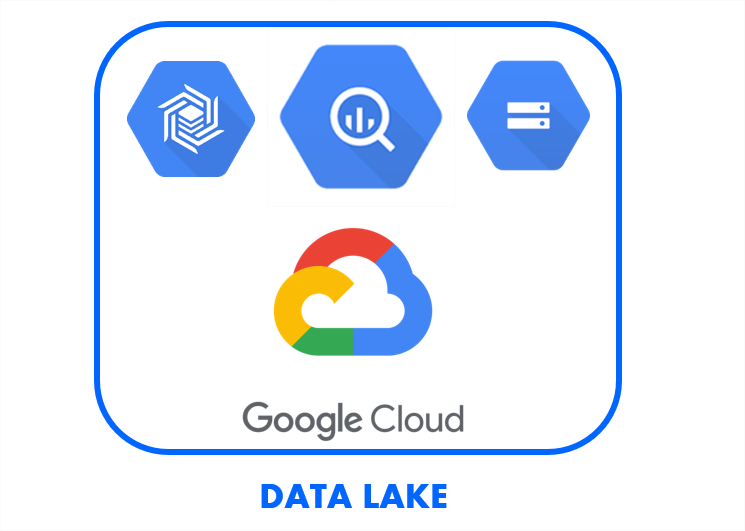
\includegraphics[width=8cm]{./images/google.png} 
\end{center}
\item IBM: IBM has collaborated with Cloudera to offer enterprise products for building a data lake and then managing, mastering, accessing, and analyzing big data.
\begin{center}
	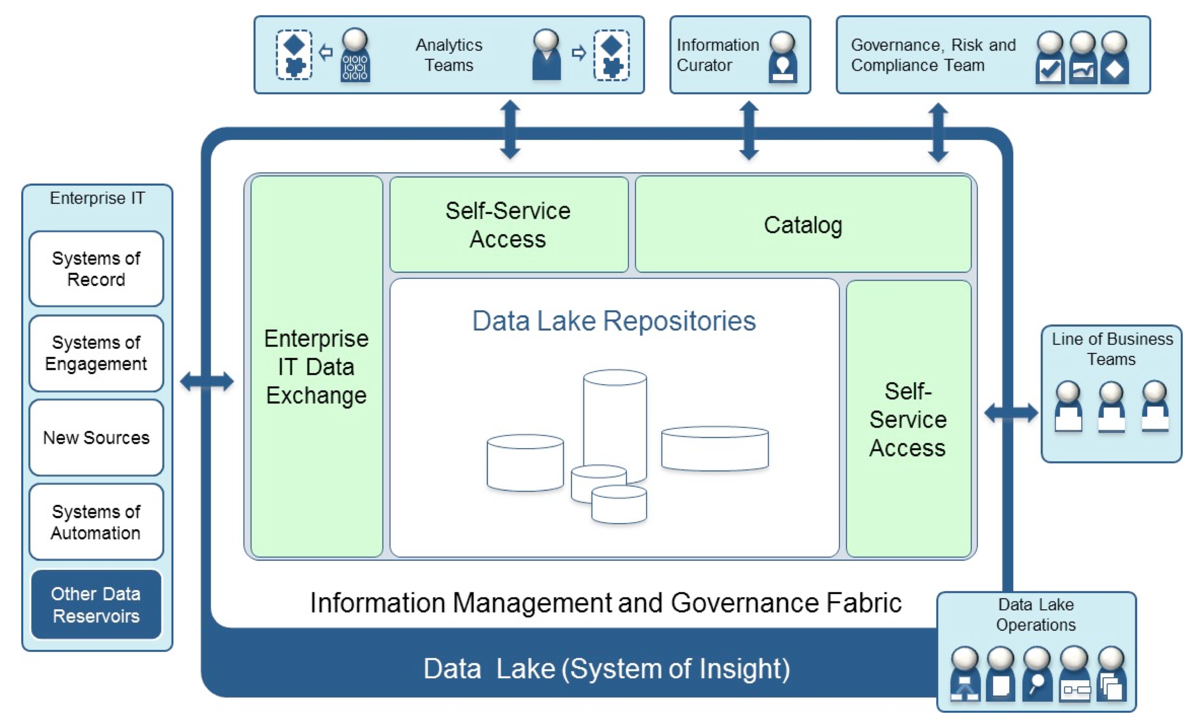
\includegraphics[width=8cm]{./images/IBM.png} 
\end{center}
\end{itemize}

 



\subsection{Datawarehouse vs Data Lake}
A data lake vs data warehouse comparison is not a competitive one because a data lake is not a direct replacement for a data warehouse; they are supplemental technologies that serve different use cases with some overlap. Most organizations that have a data lake will also have a data warehouse.
\\\
\\\
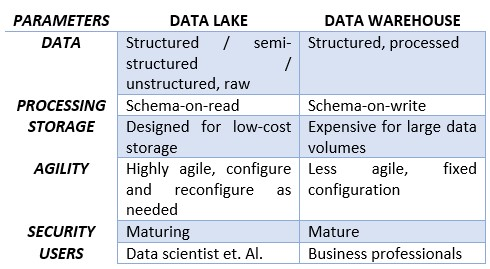
\includegraphics[width=7.5cm]{images/vs.jpg}





\section{Conclusions}
\begin{itemize}
    \item Both Data Warehouses and Data Lakes are intended to coexist in companies that wish to base their decisions on data. As you may have understood, both are complementary, not substitutes, being able to help any business to better understand the market and the consumer, in order to be able to carry out strategies based on their knowledge, with increasingly personalized communications, that is, being more customer-centric.
    
    \item The Data Warehouse provides you with cleaner, more structured and reliable results. However, in the Data Lake, by having raw and unstructured data, when making queries, users who are not very qualified, will receive quick information, but not entirely accurate, just as they would obtain it from a Data Warehouse.
    
    \item A Data Lake supports all types of data, that is, all data is stored in it, regardless of its source and structure, and it is also kept in its raw form, transforming it only when it is going to be used. In the Data Warehouse the stored data is much more critical for business and reporting.

    
\end{itemize}
 

\section{Recommendations}
\begin{itemize}
    \item Many times we can find important data sources in papers, agendas, emails and memos. The great challenge will be to figure out how to collect all this information. To achieve full knowledge of how to accumulate and process information, a close interaction with the users who are going to use the Data Warehouse within the company is essential.
    
    \item If you have been scared when you realized the vulnerability faced by data storage and you want to become a professional in it, it is recommended to use the Master in Data Science since it is the best tool you can count on.

    
\end{itemize}
\end{multicols}
\newpage


\begin{thebibliography}{}

    \bibitem{DOC2008} 
    SPEC (2021, 02 de Agosto) Data Lake vs Data Warehouse: Comparing Two Popular Data Storage - https://www.spec-india.com/blog/data-lake-vs-data-warehouse
    
    \bibitem{FRE2016} 
    MATILLION (2020, 15 de Marzo) Data Lake vs Data Warehouse - 5 Key Differences Between Both - https://www.matillion.com/resources/blog/5-key-differences-between-a-data-lake-vs-data-warehouse
   
    \bibitem{FRE2019} 
    Botelho, B. (2020, 21 de Diciembre) Data warehouse vs. data lake: Key differences - https://www.techtarget.com/searchdatamanagement/feature/Beyond-the-RDBMS-Data-warehouse-vs-data-lake-vs-data-mart
  
    \bibitem{FRE2019}
    Striim (2020) Data Warehouse vs. Data Lake vs. Data Lakehouse: An Overview of Three Cloud Data Storage Patterns - https://www.striim.com/blog/data-warehouse-vs-data-lake-vs-data-lakehouse-an-overview/
    
    \bibitem{FRE2018}
    Mobilise (2021, 10 de Mayo) Data Warehouse vs Data Lake | How They Compare - https://www.mobilise.cloud/data-warehouse-vs-data-lake/
   
   \bibitem{FRE2018}
   Chatterjee (2021) A comparative Study on Data Warehouse vs Data Lake vs Data Mart - https://www.linkedin.com/pulse/comparative-study-data-warehouse-vs-lake-mart-satrajit-chatterjee/
   
   \bibitem{FRE2018}
   Talend (2019) Data Lake vs Data Warehouse - https://www.talend.com/resources/data-lake-vs-data-warehouse/
    
    \bibitem{FRE2018}
    Taylor, David. (2022, 26 de Febrero) Data Lake vs Data Warehouse: What’s the Difference? - https://www.guru99.com/data-lake-vs-data-warehouse.html

    

 
    \end{thebibliography}
    
    


\end{document}



